\section{Ensemble Network}
 Ensembling consists of pooling together the predictions of a set of different models to produce better predictions. Nowadays, in every machine learning competitions, in particular on Kaggle, the winners use very large ensembles of models that inevitably beat any single model, no matter how good, hence we decided to use it also in our project.
 
 
Ensembling relies on the assumption that different well-performing models trained independently are likely to be good for different reasons: each model looks at slightly different aspects of the data to make its predictions, getting part of the “truth” but not all of it\footnote{This can be see in detail in the "data visualization" chapter}. By pooling the perspective of different models together, a far more accurate description of the data can be obtained.

\subsection{Our approach}
In our project we decided to use a simple ensembling approach, which is \textit{average voting}: average voting computes the average of the scores (i.e., softmax output) of the base classifiers and select the class with the highest score.

Although we decided to use this simple approach, even if it is very common, we decided to optimize the choice of models to be used in order to maximize the accuracy obtained on the validation set. In fact, all the models described in the chapter "pre-trained models" have been saved as \textit{".keras"} models so that they can be reloaded and used to directly evaluate the validation set in the ensemble, so that they do not need to be trained again (thus increasing the speed of test execution).

The main problem was to choose which of these models combined together obtained the best accuracy. Since the number of models was more than 20 a grid search seemed too slow as a method of solving this problem, so we decided to use a genetic algorithm to solve the problem automatically.

Anyway, due to the fact that we have different inputs for each type of network (ResNet, VGG and Inception) we decided to divide the ensembling networks into three types, one for each type of network.

After each genetic solution, we tested the network obtained on the test set in order to see the improvement we have on an unseen set, as we did in the previous Sections.


\subsubsection{The Ensemble Classes}
To perform the ensemble in an orderly fashion, what was done was to create three classes called respectively \textit{EnsembleVGG}, \textit{EnsembleResNet} and \textit{EnsembleInception}. The classes allows to construct an ensemble method based on a subset or the entire set of network provided to it, and evaluate the obtained network using the \textit{Keras} function \textit{evaluate}.

The class for VGG16 models is as follows:

\begin{python}
class EnsembleVGG:
    def __init__(self, set_vgg):
        self.set_vgg = set_vgg

        # create list of models
        self.model_list = []

        base_dir = '/content/drive/MyDrive/Fazzari_Ramo/Models/'
        # VGG16
        for name in vgg16:
            tmp = ks.models.load_model(base_dir + 'vgg16/' + name)
            tmp._name = name
            for i, layer in enumerate(tmp.layers):
                layer.trainable = False
                layer._name = 'ensemble_' + str(i + 1) + '_' + layer.name
            self.model_list.append(ks.models.load_model(base_dir + 'vgg16/' + name))


    def ensembleModel(self, active_models):
        models = []
        for i, model in enumerate(self.model_list):
            if active_models[i] == 1:
                model._name = str(i)
                models.append(model)
        model_input = ks.Input(shape=(IMAGE_WIDTH_VGG, IMAGE_HEIGHT_VGG, 3))
        model_outputs = [model(model_input) for model in models]
        ensemble_output = ks.layers.Average()(model_outputs)
        ensemble_model = ks.Model(inputs=model_input, outputs=ensemble_output)
        ensemble_model.compile(metrics=['accuracy'])
        return ensemble_model

    def evaluate(self, ensemble_model):
        loss, acc = ensemble_model.evaluate(self.set_vgg)
        return acc

    def ensemble_and_evaluate(self, active_models):
        if np.sum(active_models) == 0:
            return 0.0
        elif np.sum(active_models) == 1:
            print(active_models.index(1))
            return self.evaluate(self.model_list[active_models.index(1)])
        else:
            return self.evaluate(self.ensembleModel(active_models))

    def models_len(self):
        return len(self.model_list)
\end{python}

The class related to the ResNet family of networks is as follows:

\begin{python}
class EnsembleResNet:
    def __init__(self, set_resnet):
        self.set_resnet = set_resnet

        # create list of models
        self.model_list = []

        base_dir = '/content/drive/MyDrive/Fazzari_Ramo/Models/'
        # ResNet
        resnet = resnet50 + resnet101
        for i, name in enumerate(resnet):
            if i < len(resnet50):
                tmp = ks.models.load_model(base_dir + 'resnet50/' + name)
            else:
                tmp = ks.models.load_model(base_dir + 'resnet101/' + name)
            tmp._name = name
            for j, layer in enumerate(tmp.layers):
                layer.trainable = False
                layer._name = 'ensemble_' + str(j + 1) + '_' + layer.name

            self.model_list.append(tmp)



    def ensembleModel(self, active_models):
        models = []
        for i, model in enumerate(self.model_list):
            if active_models[i] == 1:
                model._name = str(i)
                models.append(model)
        model_input = ks.Input(shape=(IMAGE_WIDTH_RESNET, IMAGE_HEIGHT_RESNET, 3))
        model_outputs = [model(model_input) for model in models]
        ensemble_output = ks.layers.Average()(model_outputs)
        ensemble_model = ks.Model(inputs=model_input, outputs=ensemble_output)
        ensemble_model.compile(metrics=['accuracy'])
        return ensemble_model

    def evaluate(self, ensemble_model):
        loss, acc = ensemble_model.evaluate(self.set_resnet)
        return acc

    def ensemble_and_evaluate(self, active_models):
        if np.sum(active_models) == 0:
            return 0.0
        elif np.sum(active_models) == 1:
            print(active_models.index(1))
            return self.evaluate(self.model_list[active_models.index(1)])
        else:
            return self.evaluate(self.ensembleModel(active_models))

    def models_len(self):
        return len(self.model_list)
\end{python}

Finally, the ensemble class for Inception is:

\begin{python}
class EnsembleInception:
    def __init__(self, set_inception):
        self.set_inception = set_inception

        # create list of models
        self.model_list = []

        base_dir = '/content/drive/MyDrive/Fazzari_Ramo/Models/'
        # VGG16
        for name in inception:
            tmp = ks.models.load_model(base_dir + 'inception/' + name)
            tmp._name = name
            for i, layer in enumerate(tmp.layers):
                layer.trainable = False
                layer._name = 'ensemble_' + str(i + 1) + '_' + layer.name
            self.model_list.append(ks.models.load_model(base_dir + 'inception/' + name))


    def ensembleModel(self, active_models):
        models = []
        for i, model in enumerate(self.model_list):
            if active_models[i] == 1:
                model._name = str(i)
                models.append(model)
        model_input = ks.Input(shape=(IMAGE_WIDTH_INCEPTION, IMAGE_HEIGHT_INCEPTION, 3))
        model_outputs = [model(model_input) for model in models]
        ensemble_output = ks.layers.Average()(model_outputs)
        ensemble_model = ks.Model(inputs=model_input, outputs=ensemble_output)
        ensemble_model.compile(metrics=['accuracy'])
        return ensemble_model

    def evaluate(self, ensemble_model):
        loss, acc = ensemble_model.evaluate(self.set_inception)
        return acc

    def ensemble_and_evaluate(self, active_models):
        if np.sum(active_models) == 0:
            return 0.0
        elif np.sum(active_models) == 1:
            print(active_models.index(1))
            return self.evaluate(self.model_list[active_models.index(1)])
        else:
            return self.evaluate(self.ensembleModel(active_models))

    def models_len(self):
        return len(self.model_list)
\end{python}

The constructor takes as input the testset for which the ensemble class will do the evaluation, and what it does is load the different models. Next, in each three we have four functions:

\begin{enumerate}
	\item \textit{ensembleModel}: given an array of equal size to the number of different models, the function creates an ensemble model using the models that are in the position where in the input array there is a one.
	\item \textit{evaluate}: calls the keras evaluate function on the ensemble model
	\item \textit{ensemble\_and\_evaluate}: calls both the ensembleModel and the evaluate functions. In cases the input is all made of zeros, it returns 0 without further computations, on the other hand if the input has only one 1 in it the function evaluates it directly.
	\item \textit{models\_len}: retrieves the number of models.
\end{enumerate}

Notice that in all functions we modified the name of the layers and models in order to prevent every form of name duplication in the ensemble network.  

\subsubsection{Genetic Algorithm Workflow}
Following the guidelines in Section 2.6, we need to decide how to develop the different components and decide on the hyperparameters in order to define the flow of the genetic algorithm.

\paragraph{Genotype}
In our specific case, our chromosomes are binary encoded and each gene represents a different model. Hence, we have individuals made of a number of genes equal to the number of different models that we have.

\begin{python}
# create an operator that randomly returns 0 or 1
toolbox.register('zeroOrOne', random.randint, 0, 1)

# define a single objective, maximizing fitness strategy:
creator.create('FitnessMax', base.Fitness, weights=(1.0,))

# create the Individual class based on list:
creator.create('Individual', list, fitness=creator.FitnessMax)

# create the individual operator to fill up an Individual instance:
toolbox.register('individualCreator', tools.initRepeat, creator.Individual, toolbox.zeroOrOne, INDIVIDUAL_LENGTH)
\end{python}

\paragraph{Population}
The population is composed of 8 individuals, we decided to keep the number of individuals low so as to reduce the number of evaluations done and, therefore, the total duration of the algorithm, in order to obtain a satisfactory result by waiting less than an hour.

\begin{python}
toolbox.register('populationCreator', tools.initRepeat, list, toolbox.individualCreator)
\end{python}

\paragraph{Fitness Function}
The fitness function is the accuracy obtained through the \textit{predict\_and\_evaluate} function of the Ensemble class. It was registered in the \textit{toolbox} as follows:

\begin{python}
def ensembleAccuracy(individual):
    return ensemble.predict_and_evaluate(individual),

toolbox.register('evaluate', ensembleAccuracy)
\end{python}

Notice that the function returns a tuple, this is done because the framework accept only tuple values as result of the evaluation function.
\paragraph{Selection Algorithm}
The selection algorithm used in this case is \textit{tournament selection}. In each round of the tournament selection method, two individuals are randomly picked from the population, and the one with the highest fitness score wins and gets selected. We decided to select only two individuals since our population is small and selecting more could cause an abuse in exploitation.

\begin{python}
# Tournament selection with tournament size of 2:
toolbox.register("select", tools.selTournament, tournsize=2)
\end{python}


\paragraph{Crossover Algorithm}
As crossover algorithm we decided to use the \textit{two-point crossover}. In the two-point crossover method, two crossover points on the chromosomes of both parents are selected randomly. The genes residing between these points are swapped between the two parent chromosomes.

The following diagram demonstrates a two-point crossover carried out on a pair of binary chromosomes, with the first crossover point located between the third and fourth genes, and the other between the seventh and eighth genes:

\begin{figure}[H]
	\centering
	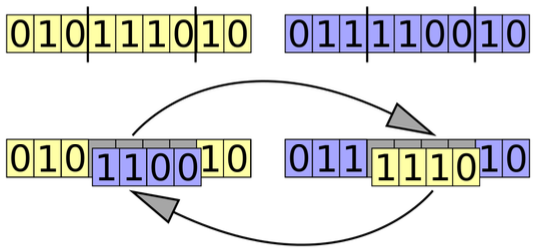
\includegraphics[width=0.4\textwidth]{img/twopointcross.png}
	\caption{Two point crossover example.}
	\label{fig:twopointcross}
\end{figure}

The code for that is:
\begin{python}
toolbox.register("mate", tools.cxTwoPoint)
\end{python}

\paragraph{Mutation Algorithm}
As mutation algorithm we decided to use the \textit{Multiple Flip bit mutation}. When applying the flip bit mutation to a binary chromosome, one gene is randomly selected and its value is flipped (complemented), as shown in the following diagram:

\begin{figure}[H]
	\centering
	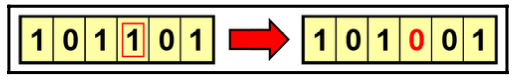
\includegraphics[width=0.4\textwidth]{img/flipbit.png}
	\caption{Flip bit mutation example.}
	\label{fig:flipbit}
\end{figure}

This can be extended to several random genes being flipped instead of just one, obtaining the multiple flip bit mutation that we use.
The code for that is:
\begin{python}
toolbox.register("mutate", tools.mutFlipBit, indpb=1.0/INDIVIDUAL_LENGTH)
\end{python}


\paragraph{Elitism}
We set the number of individuals for the elitism mechanism to 1. This value was decided to have a minimum of elitism, but without abusing it too much. In fact, the number of individuals is so low that having a higher value could lead to a problem, therefore, in order not to risk bad results (i.e., not global optimum results), we chose to use this conservative approach and limit the number to only one.

\paragraph{GA Flow}
The first thing to do is to define the initial population, this is easily done by the following line of code:

\begin{python}
population  = toolbox.populationCreator(n=POPULATION_SIZE)
\end{python}

After that, we created a statistical object. This object has served to have a report of the flow of the genetic algorithm, allowing us to save for each generation the maximum and average fitness values obtained, so that we can show them once the generations are over.

\begin{python}
stats = tools.Statistics(lambda ind: ind.fitness.values)
stats.register("max", np.max)
stats.register("avg", np.mean)
\end{python}

Then, the last object we need to create for the \textit{eaSimple} is the \textbf{HallOfFame}, which can be done through the following line of code:

\begin{python}
hof = tools.HallOfFame(HALL_OF_FAME_SIZE)
\end{python}

The main flow is done using the \textit{eaSimple} in the way as follow:

\begin{python}
population, logbook = eaSimpleWithElitism(population,
								  toolbox,
								  cxpb=P_CROSSOVER,
								  mutpb=P_MUTATION,
								  ngen=MAX_GENERATIONS,
								  stats=stats,
								  halloffame=hof,
								  verbose=True)
\end{python}

Where the P\_CROSSOVER is equal to 0.9, P\_MUTATION 0.1.\footnote{Value suggested by the book ”Hands on Genetic Algorithms with Python” by Eyal Wirsansky, also the other values of probabilities are taken by the suggestions of the book}



\subsubsection{GA Results for VGG16 Ensemble}
The following graph shows the results obtained for each generation from the population (i.e., the maximum and mean accuracy):

\begin{figure}[H]
	\centering
	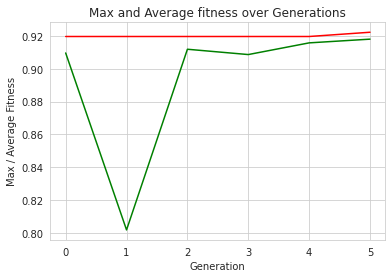
\includegraphics[width=0.4\textwidth]{img/ensemble/vgg.png}
	\caption{Maximum and average accuracy in the population for each generation.}
	\label{fig:ensemblevgg}
\end{figure}


As it can be noticed from the graph the elitism allows the maximum value to never go down. Moreover, it is possible to notice that the maximum result obtained is much higher than the one obtained with VGG16, which reached almost 80\%, instead here we reach 92.23\%. This was obtained from the genetic algorithm by combining the following models together:
 \begin{itemize}
	\item VGG16 feature extraction
	\item VGG16 feature extraction with dropout
	\item VGG16 with 2 layers finetuned and with dropout
         \item VGG16 with 1 layer finetuned
\end{itemize}
Chosen by the chromosome [0, 0, 1, 1, 1, 1, 0], our winner in the final population.

Looking closely at the graph we can see a very slight growth at the end of the fifth generation, this with later testing turned out to be the global optimum.

Testing the network obtained by choosing the above models with the test set it was possible to obtain an accuracy of 0.9586. Very high and even higher than that obtained on the validation set, this can be related to two reasons:

\begin{enumerate}
	\item The features of the frameworks in the test set are much more similar to those in the training, possible but not that much;
	\item The quantity of pictures present in the test set is greater than that of the validation as reported in chapter 1.2, therefore the weight of mistaking a picture in the case of validation has a higher weight in percentage than in the test set.
\end{enumerate}




\subsubsection{GA Results for ResNet Ensemble}
The following graph shows the results obtained for each generation from the population (i.e., the maximum and mean accuracy):

\begin{figure}[H]
	\centering
	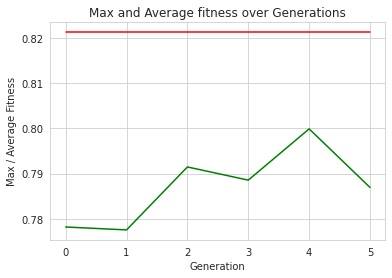
\includegraphics[width=0.4\textwidth]{img/ensemble/resnet.png}
	\caption{Maximum and average accuracy in the population for each generation.}
	\label{fig:ensembleresnet}
\end{figure}

The maximum accuracy value for ResNet was obtained in Section 4.2.4 using fine tuning of one block and two additional dense layers at the end of the network, reaching an accuracy score of 0.6736. Also here we exceed the value reached by the single model obtaining a much higher value, reaching 0.8212, satisfactory value even if lower than the one obtained with the ensemble of VGGs. This was obtained from the genetic algorithm by combining the following models together:
 \begin{itemize}
	\item ResNet50 with 1 block finetuned 
         \item ResNet50 with 2 blocks finetuned 
         \item ResNet50 with 1 block finetuned plus two dense layers at the end of it
         \item ResNet50 with 2 blocks finetuned plus two dense layers at the end of it
	\item ResNet101 finetuned till block 4
\end{itemize}
Chosen by the chromosome [0, 1, 1, 1, 1, 0, 0, 1, 0, 0, 0, 0], our winner in the final population.

Anyway, it is important to notice here that the value for the average forms a mountain scape shape, this is a problem related to the GA hyperparameters and operators, which led to unravel the result obtained by the previous population.

Testing the network obtained by choosing the above models with the test set it was possible to obtain an accuracy of 0.9517. Very high and much higher than that obtained on the validation set, hence we can take into consideration the hypothesis done, related to this behavior, in the previous paragraph.


\subsubsection{GA Results for ResNet Inception}
The following graph shows the results obtained for each generation from the population (i.e., the maximum and mean accuracy):

\begin{figure}[H]
	\centering
	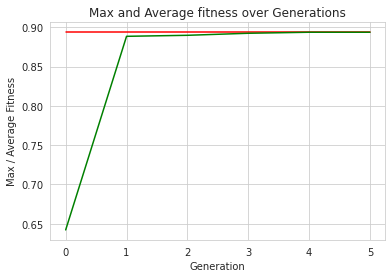
\includegraphics[width=0.4\textwidth]{img/ensemble/inception.png}
	\caption{Maximum and average accuracy in the population for each generation.}
	\label{fig:ensembleinception}
\end{figure}

The maximum accuracy value for Inception was obtained in Section 4.4.5 fine tuning 3 blocks and using exponential decay for the learning rate, reaching an accuracy score of 0.5803. Also here we exceed the value reached by the single model obtaining a much higher value, reaching 0.8938, satisfactory value even if lower than the one obtained with the ensemble of VGGs. This was obtained from the genetic algorithm by combining the following models together:
 \begin{itemize}
	\item Inception with 1 block finetuned
	\item Inception with 3 blocks finetuned
\end{itemize}
Chosen by the chromosome [0, 1, 0, 1, 0], our winner in the final population.

Testing the network obtained by choosing the above models with the test set it was possible to obtain an accuracy of 0.9264 and a loss equal to 0.3 (in the other ensembles it was really close to 0 that the evaluation function of keras printed directly 0). Very high and much higher than that obtained on the validation set, hence we can take into consideration the hypothesis done, related to this behavior, in the previous paragraph.


